\documentclass[border=10pt,tikz]{standalone}
\usepackage{tikz}
\usetikzlibrary{positioning,arrows.meta,shapes}
\begin{document}
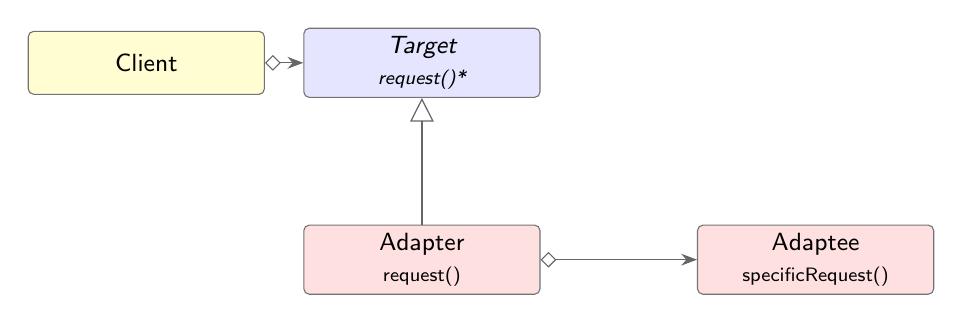
\begin{tikzpicture}[
  font=\sffamily\small,
  cls/.style={rectangle, rounded corners=2pt, draw=black!55, line width=0.4pt,
              minimum height=8mm, minimum width=30mm, inner sep=3pt, fill=white, align=center},
  abs/.style={cls, fill=blue!10, font=\sffamily\itshape\small},
  con/.style={cls, fill=red!12},
  cli/.style={cls, fill=yellow!18},
  inh/.style={-{Triangle[length=3mm,width=3mm,open]}, draw=black!60, line width=0.45pt},
  agg/.style={{Diamond[length=2mm,width=2mm,open]}-{Stealth[length=2mm]}, draw=black!60}
]
\node[cli] (c)   at (-4.5, 0) {Client};
\node[abs] (t)   at (-1, 0)   {Target \\ \scriptsize request()*};
\node[con] (a)   at (-1,-2.5) {Adapter \\ \scriptsize request()};
\node[con] (e)   at ( 4,-2.5) {Adaptee \\ \scriptsize specificRequest()};

\draw[agg] (c.east) -- (t.west);
\draw[inh] (a.north) -- (t.south);
\draw[agg] (a.east) -- (e.west);
\end{tikzpicture}
\end{document}
